\subsection{Cosmic Radiation Results}
\label{sec:Cosmic-Radiation-Results}

The FITPix recorded a total of 15810 frames, and the MiniPIX recorded a total of 15735 frames.
As can be seen by comparing Figures \ref{subfig:minipix-counts} and \ref{subfig:fitpix-counts}, the MiniPIX and FITPix recorded a similar number of counts throughout the duration of flight.
Their dose measurements are slightly different in value due to the difference in energy threshold between the two detectors, but the plots follow the same trend.
These results are also comparable to the data recorded during the 2018 SORA flight, which can be seen in Figure \ref{fig:2018-minipix-data}.

\begin{figure}[h!]
\hfill
\subfigure[MiniPIX counts measured during flight.]{\label{subfig:minipix-counts}\includegraphics[width=8cm]{figures/mp_counts.pdf}}
\hfill
\subfigure[MiniPIX dose measure during flight.]{\label{subfig:minipix-dose}\includegraphics[width=8cm]{figures/mp_dose.pdf}}
\hfill
\caption{MiniPIX particle data detected during flight.}
\label{fig:minipix-data}
\end{figure}

\begin{figure}[h!]
\hfill
\subfigure[FITPix counts measured during flight.]{\label{subfig:fitpix-counts}\includegraphics[width=8cm]{figures/fp_counts.pdf}}
\hfill
\subfigure[FITPix dose measure during flight.]{\label{subfig:fitpix-dose}\includegraphics[width=8cm]{figures/fp_dose.pdf}}
\hfill
\caption{MiniPIX particle data detected during flight.}
\label{fig:fitpix-data}
\end{figure}

\begin{figure}[h!]
	\begin{center}
	\includegraphics[width=0.95\textwidth]{figures/counts_per_second_2018.pdf}
	\caption{Counts from the 2018 SORA mission.}
	\label{fig:2018-minipix-data}
	\end{center}
\end{figure}

\begin{figure}[h!]
\subfigure[Histogram of the LET from each cluster type collected by the MiniPIX during flight.]{\includegraphics[width=12cm]{figures/mp_track_let_histogram.pdf}}
\hfill
\subfigure[Density plot of the LET from each cluster type collected by the MiniPIX during flight.]{\includegraphics[width=12cm]{figures/mp_track_let_density.pdf}}
\hfill
\caption{MiniPIX LET distributions from flight data.}
\label{fig:minipix-let}
\end{figure}

\begin{figure}[h!]
\subfigure[Histogram of the LET from each cluster type collected by the FITPix during flight.A logarithmic scale was used for the y-axis due to the small blob counts being relatively larger than all other counts.]{\includegraphics[width=12cm]{figures/fp_track_let_histogram.pdf}}
\hfill
\subfigure[Density plot of the LET from each cluster type collected by the FITPix during flight.]{\includegraphics[width=12cm]{figures/fp_track_let_density.pdf}}
\hfill
\caption{FITPix LET distributions from flight data.}
\label{fig:fitpix-let}
\end{figure}



\begin{figure}[h!]
\subfigure[Data from photodiode 0.]{\includegraphics[width=8cm]{figures/photo_0.pdf}}
\hfill
\subfigure[Data from photodiode 1.]{\includegraphics[width=8cm]{figures/photo_1.pdf}}
\hfill
\subfigure[Data from photodiode 2.]{\includegraphics[width=8cm]{figures/photo_2.pdf}}
\hfill
\subfigure[Data from photodiode 3.]{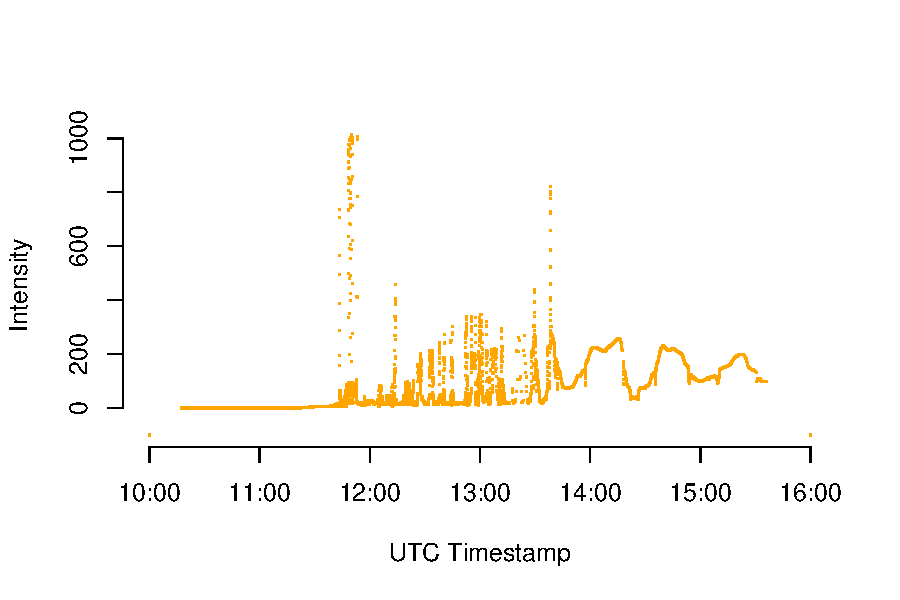
\includegraphics[width=8cm]{figures/photo_3.pdf}}
\hfill
\caption{Photodiode data from the flight.}
\label{fig:photodiodes}
\end{figure}


\subsection{Organic Solar Cell Results}
\label{sec:Solar-Cell-Results}

The main goal of the solar cell experiment was to observe changes in the structure and performance of the organic solar cells before and after being exposed to the stratosphere.
The purpose of the current reading circuit for the solar cells was mainly to provide a proof-of-concept in order to show that it is possible to easily perform the IV measurements within the context of our payload.
The current reading circuit that was flown accomplished this goal.
The data recorded by the current reading circuit was legible enough to clearly see the relationship between current produced by the cell and the voltage applied across the cell.
However, the data is not precise enough to determine values such as $V_{oc}$ or $I_{sc}$.
An IV curve that was measured using lab equipment is shown next to an example of data recorded by the current reading circuit in Figure \ref{fig:solar-cell-measurements}. 
Due to the variablility of the data recorded by our circuit, it is not possible to use this data for any calculations.
Only one plot is shown since all measurements made by the circuit look similar.
A discussion of potential improvements for this circuit can be found in Section \ref{subsec:Electronics-Discussion}.

\begin{figure}[h!]
\hfill
\subfigure[IV curve recorded by the equipment in the solar cell fabrication lab. This plot was made immediately after fabricating the cell. There had not been enough time for the cell to degrade which is why this plot is so well-defined.]{\includegraphics[width=8cm]{figures/lab-data-plot.pdf}}
\hfill
\subfigure[IV curve recorded by SORA 3's IV measuring circuit. This plot was made a considerable time after the cell was fabricated, which is why it is not very well-defined.]{\includegraphics[width=8cm]{figures/current-reader-plot.pdf}}
\hfill
\caption{IV curves measured by two different sources.}
\label{fig:solar-cell-measurements}
\end{figure}
